\documentclass[9pt,onecolumn]{article}
\usepackage[paper=a4paper,margin=0.57in]{geometry}
\usepackage[utf8]{inputenc}
\usepackage{graphicx}
\usepackage{hyperref}
\usepackage[labelfont=bf]{caption}
\usepackage{subcaption}
\usepackage{amsmath}
\usepackage{amssymb}
\usepackage{mathtools}
\usepackage{mathrsfs}
\usepackage{physics}
\usepackage[square,numbers]{natbib}
\usepackage[nameinlink,capitalise]{cleveref}
\usepackage{url}
\usepackage{xcolor}
\usepackage{authblk}
\usepackage{rotating}
\usepackage{nameref}
\usepackage{pdflscape}
\usepackage[title]{appendix}
% \usepackage[useregional]{datetime2}
\setlength{\rotFPtop}{0pt plus 1fil}
\setlength\columnsep{.4in}
%\usepackage{tabulary}  
\usepackage[switch, modulo]{lineno}
\linenumbers
\graphicspath{{Fig/Supplement/}}

\makeatletter
\let\@fnsymbol\@arabic
\makeatother
\DeclarePairedDelimiter{\ceil}{\lceil}{\rceil}
\newcommand*\mystrut[1]{\vrule width0pt height0pt depth#1\relax}
\newcommand*\twocell[3]{\begin{tabular}{#1} #2 \\ #3 \end{tabular}}
\newcommand*\threecell[4]{\begin{tabular}{#1} #2 \\ #3 \\ #4 \end{tabular}}
\newcommand*\sfn[2]{$#1 \times 10^{#2}$}
\newcommand*{\intro}{\hyperref[sec:introduction]{Introduction}}

\renewcommand{\thefigure}{S\arabic{figure}}
\renewcommand{\figurename}{Supplementary Figure}

\setcounter{figure}{0}

\setcounter{secnumdepth}{3}
\renewcommand{\thesubsection}{(\alph{subsection})}
    
\begin{document}
\title{Supplement 2: Improved population fitness in a larger habitat is reduced or even reversed by clonal interference from a zero-sum trait}
\author{Kevin Gomez, Nathan R. Aviles, Jason Bertram, and Joanna Masel}

\maketitle

\newpage
\begin{landscape}
\vspace*{\fill}
\begin{figure}[!h]
    \centering
    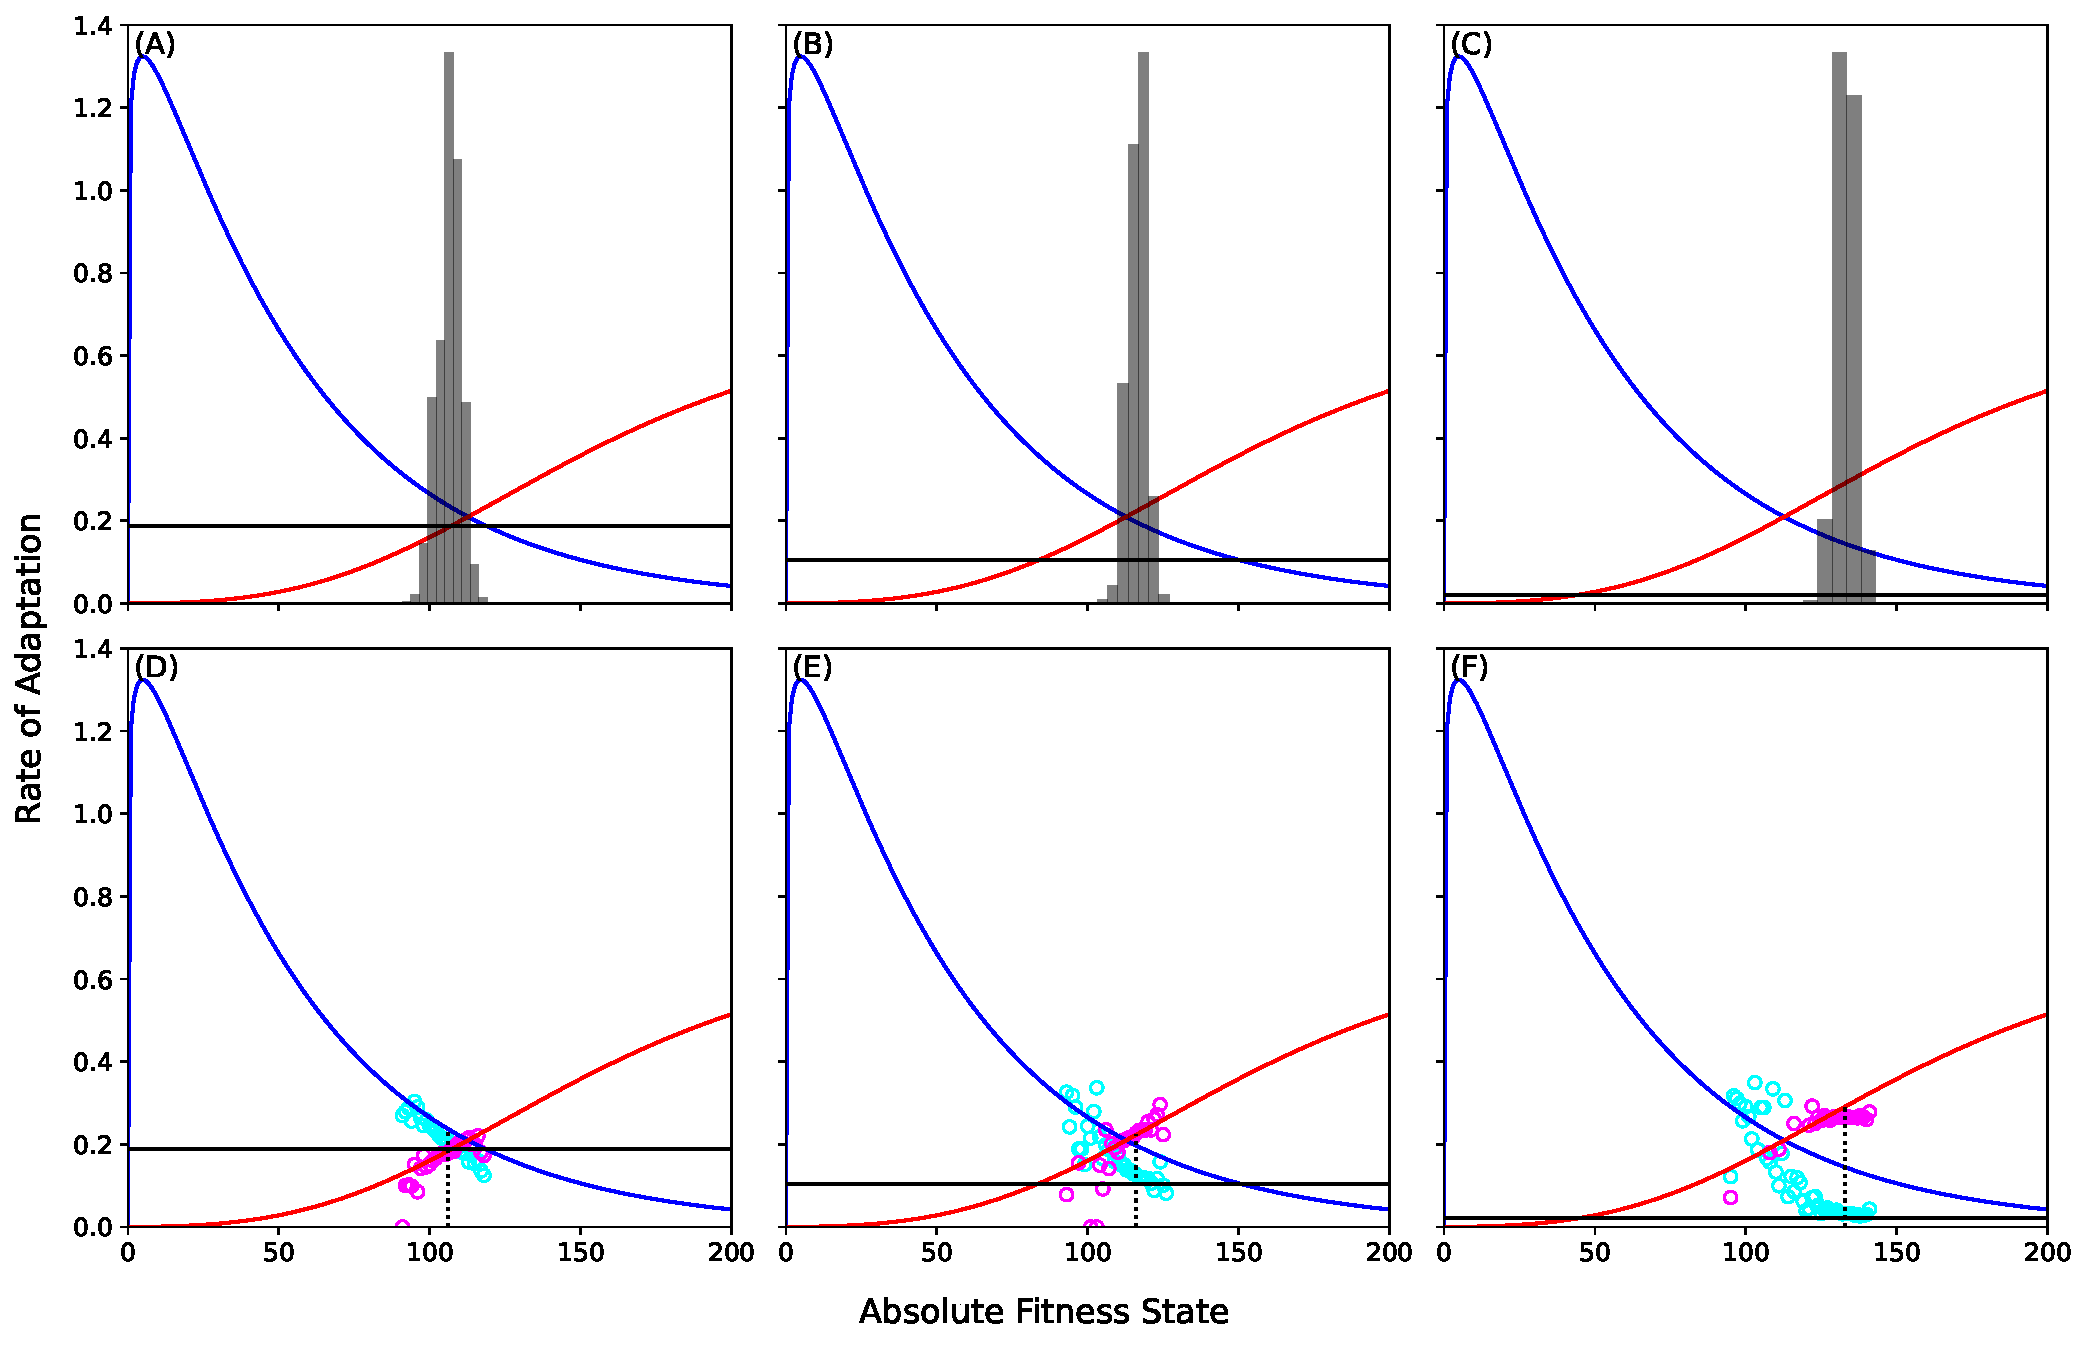
\includegraphics[scale=.60]{Fig/Supplement/fig_bEvo_DRE_traitInterference_mcPlots_pnlA.pdf}
    \caption{Imperfect stalling in simulations has only a small effect on a population's level and rates of adaptation. Top row (A-C) shows a histogram of a population's mean position in simulations, with the overall mean projected down to a dashed vertical line in (D-F).  Horizontal black lines show rapid environmental change in the left column (A, D), contrasting with slow environmental change in the right column (C, F). Rapid environmental change causes the population to fall slightly short of the level of adaptation predicted from stalling against relative adaptation (histogram in (A) is to the left of the intersection of the red and blue lines). Very slow environmental change allows the population to ratchet to slightly higher levels of adaptation than predicted by perfect stalling (histogram in (C) is to the right of the intersection of the red and blue lines). However, the population remains closer to the red-blue intersection than to the blue-black intersection that would be reached in the absence of stalling from the relative fitness trait. Simulated cyan and pink points in the bottom row (D-F) show how rates of adaptation compare to the blue and red predicted lines for adaptation in $b$ and $c$, respectively. Under perfect stalling, these would drop suddenly to zero to the right and to the left of the intersection, respectively. Falls relative to the predicted lines can be seen, but do not represent dramatic step functions. In all panels, $\rho=0.93$ with $T=10^9$, $d=1.2$, $U_b=5\times10^{-7}$, $U_c=5\times10^{-6}$, $s_{b,0}=0.03$, $\alpha=0.99$, and $c_{+}=0.02$.}
\label{fig:supp:mcSimEst_smallRho}
\end{figure}
\vspace*{\fill}\clearpage

\newpage
\vspace*{\fill}
\begin{figure}[!h]
    \centering
    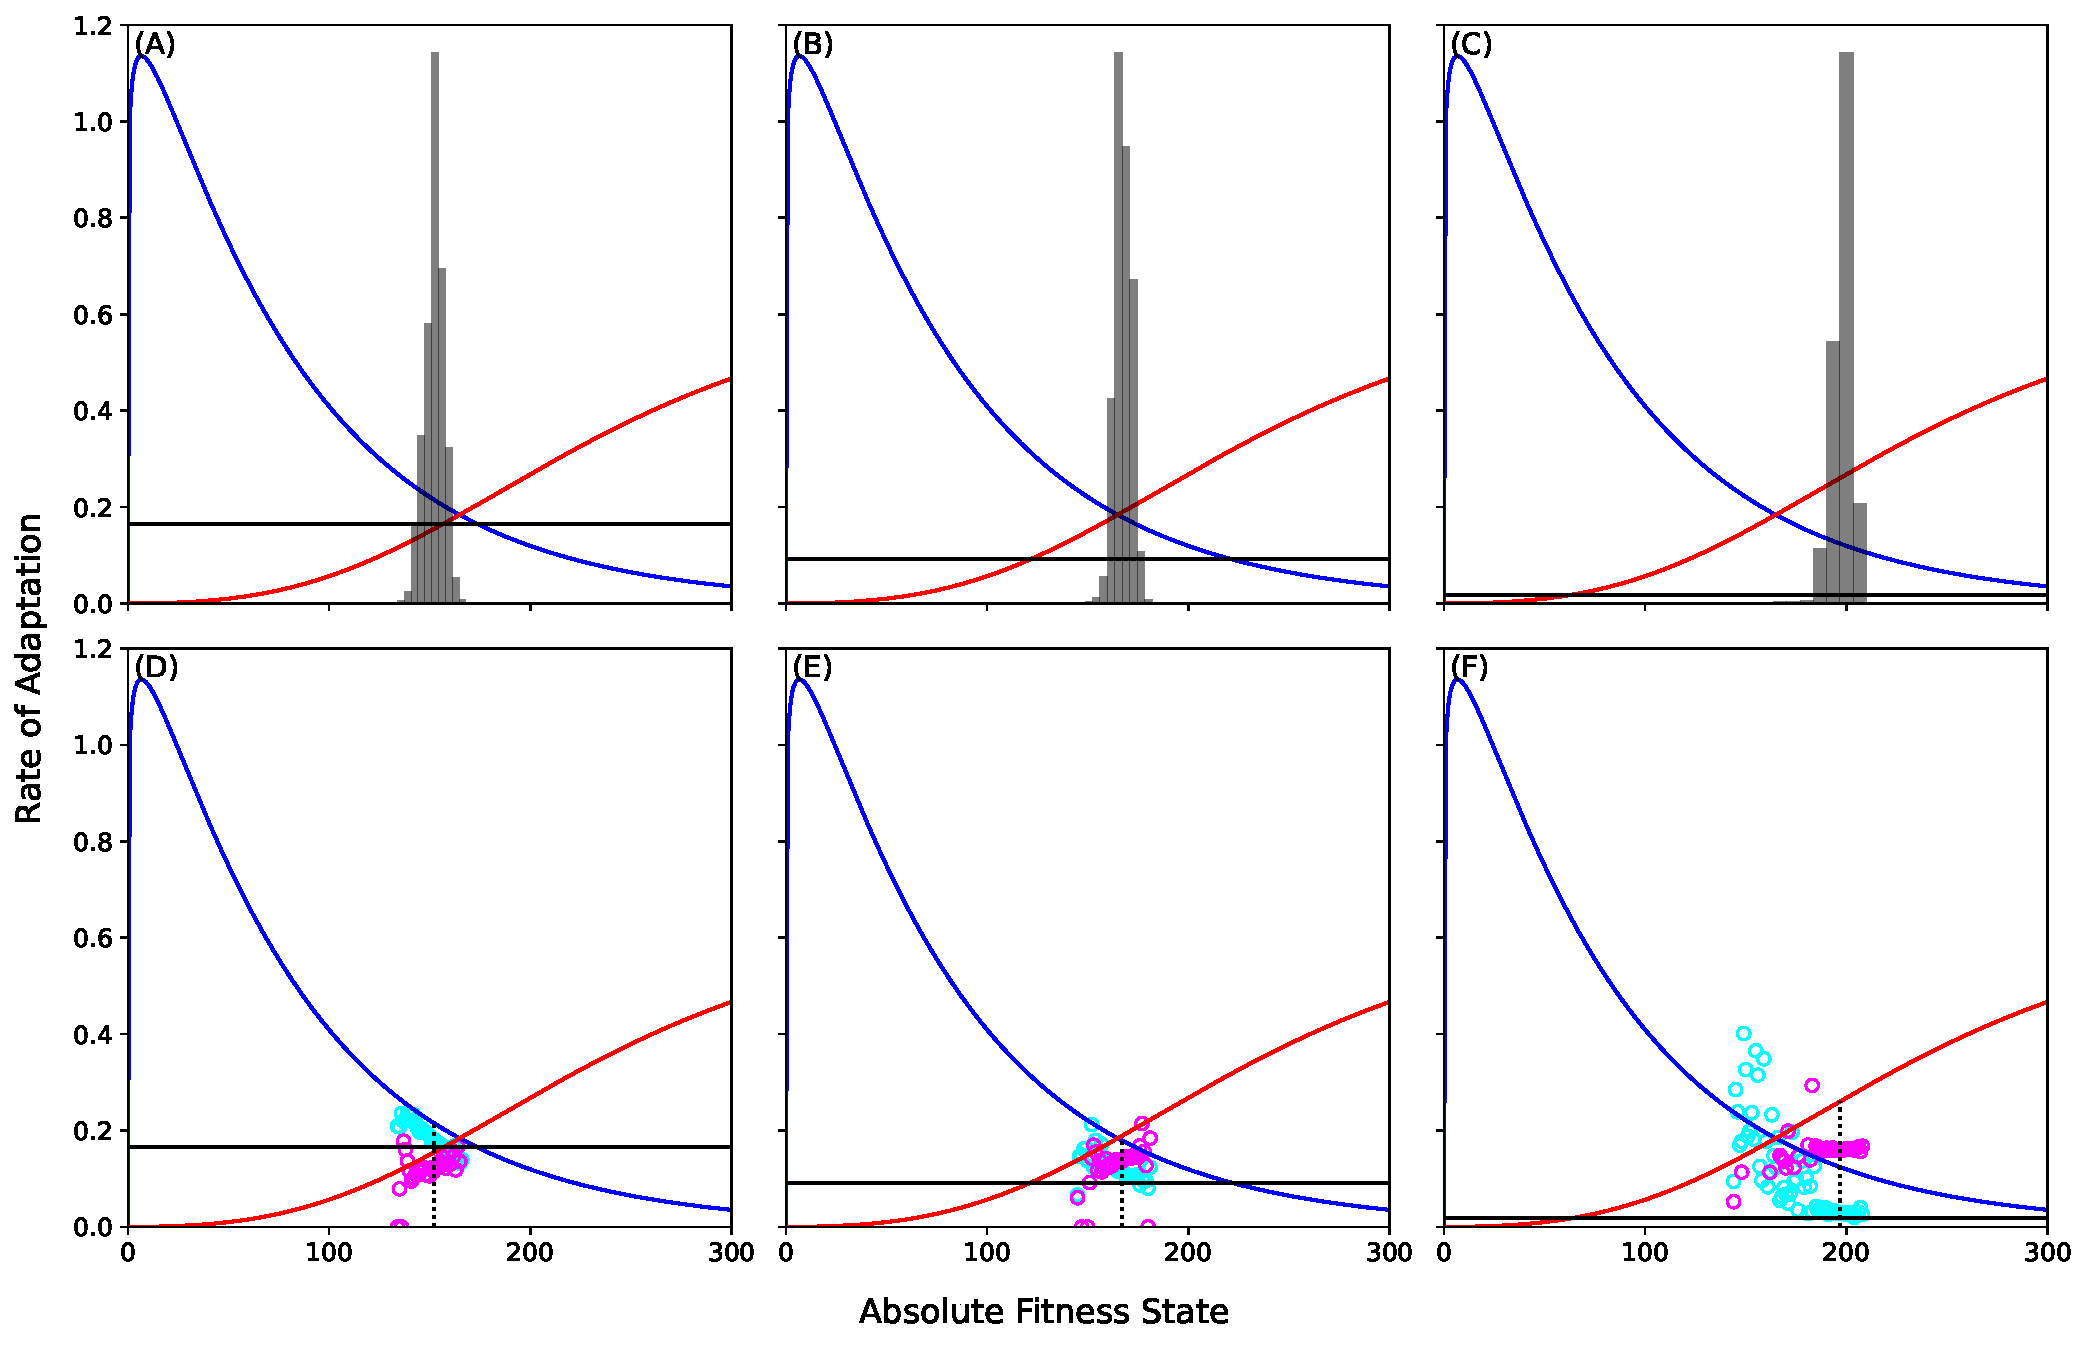
\includegraphics[scale=.60]{Fig/Supplement/fig_bEvo_DRE_traitInterference_mcPlots_pnlB.pdf}
    \caption{The degree of evolutionary stalling in the absolute fitness trait remains strong with alternate model parameters, chosen to produce a higher $\rho$. $v_b$ decays slower relative to \ref{fig:supp:mcSimEst_smallRho} due to weaker diminishing returns epistasis. We also see a more gradual decay in $v_{b,est}$, but gains in absolute fitness continue to be substantially less than those expected in the absence of stalling from the relative fitness trait. (A-E) include estimates rates of adaptation, while (F-J) provide histograms showing sojourn times of the population mean fitness state. In all panels, $\rho=1$, $T=10^9$, $d=1.2$, $U_b=5\times10^{-6}$, $U_c=5\times10^{-6}$, $s_{b,0}=0.02$, $\alpha=0.993$, and $c_{+}=0.02$.}
    \label{fig:supp:mcSimEst_mediumRho}
\end{figure}
\vspace*{\fill}\clearpage

\newpage
\vspace*{\fill}
\begin{figure}[!h]
    \centering
    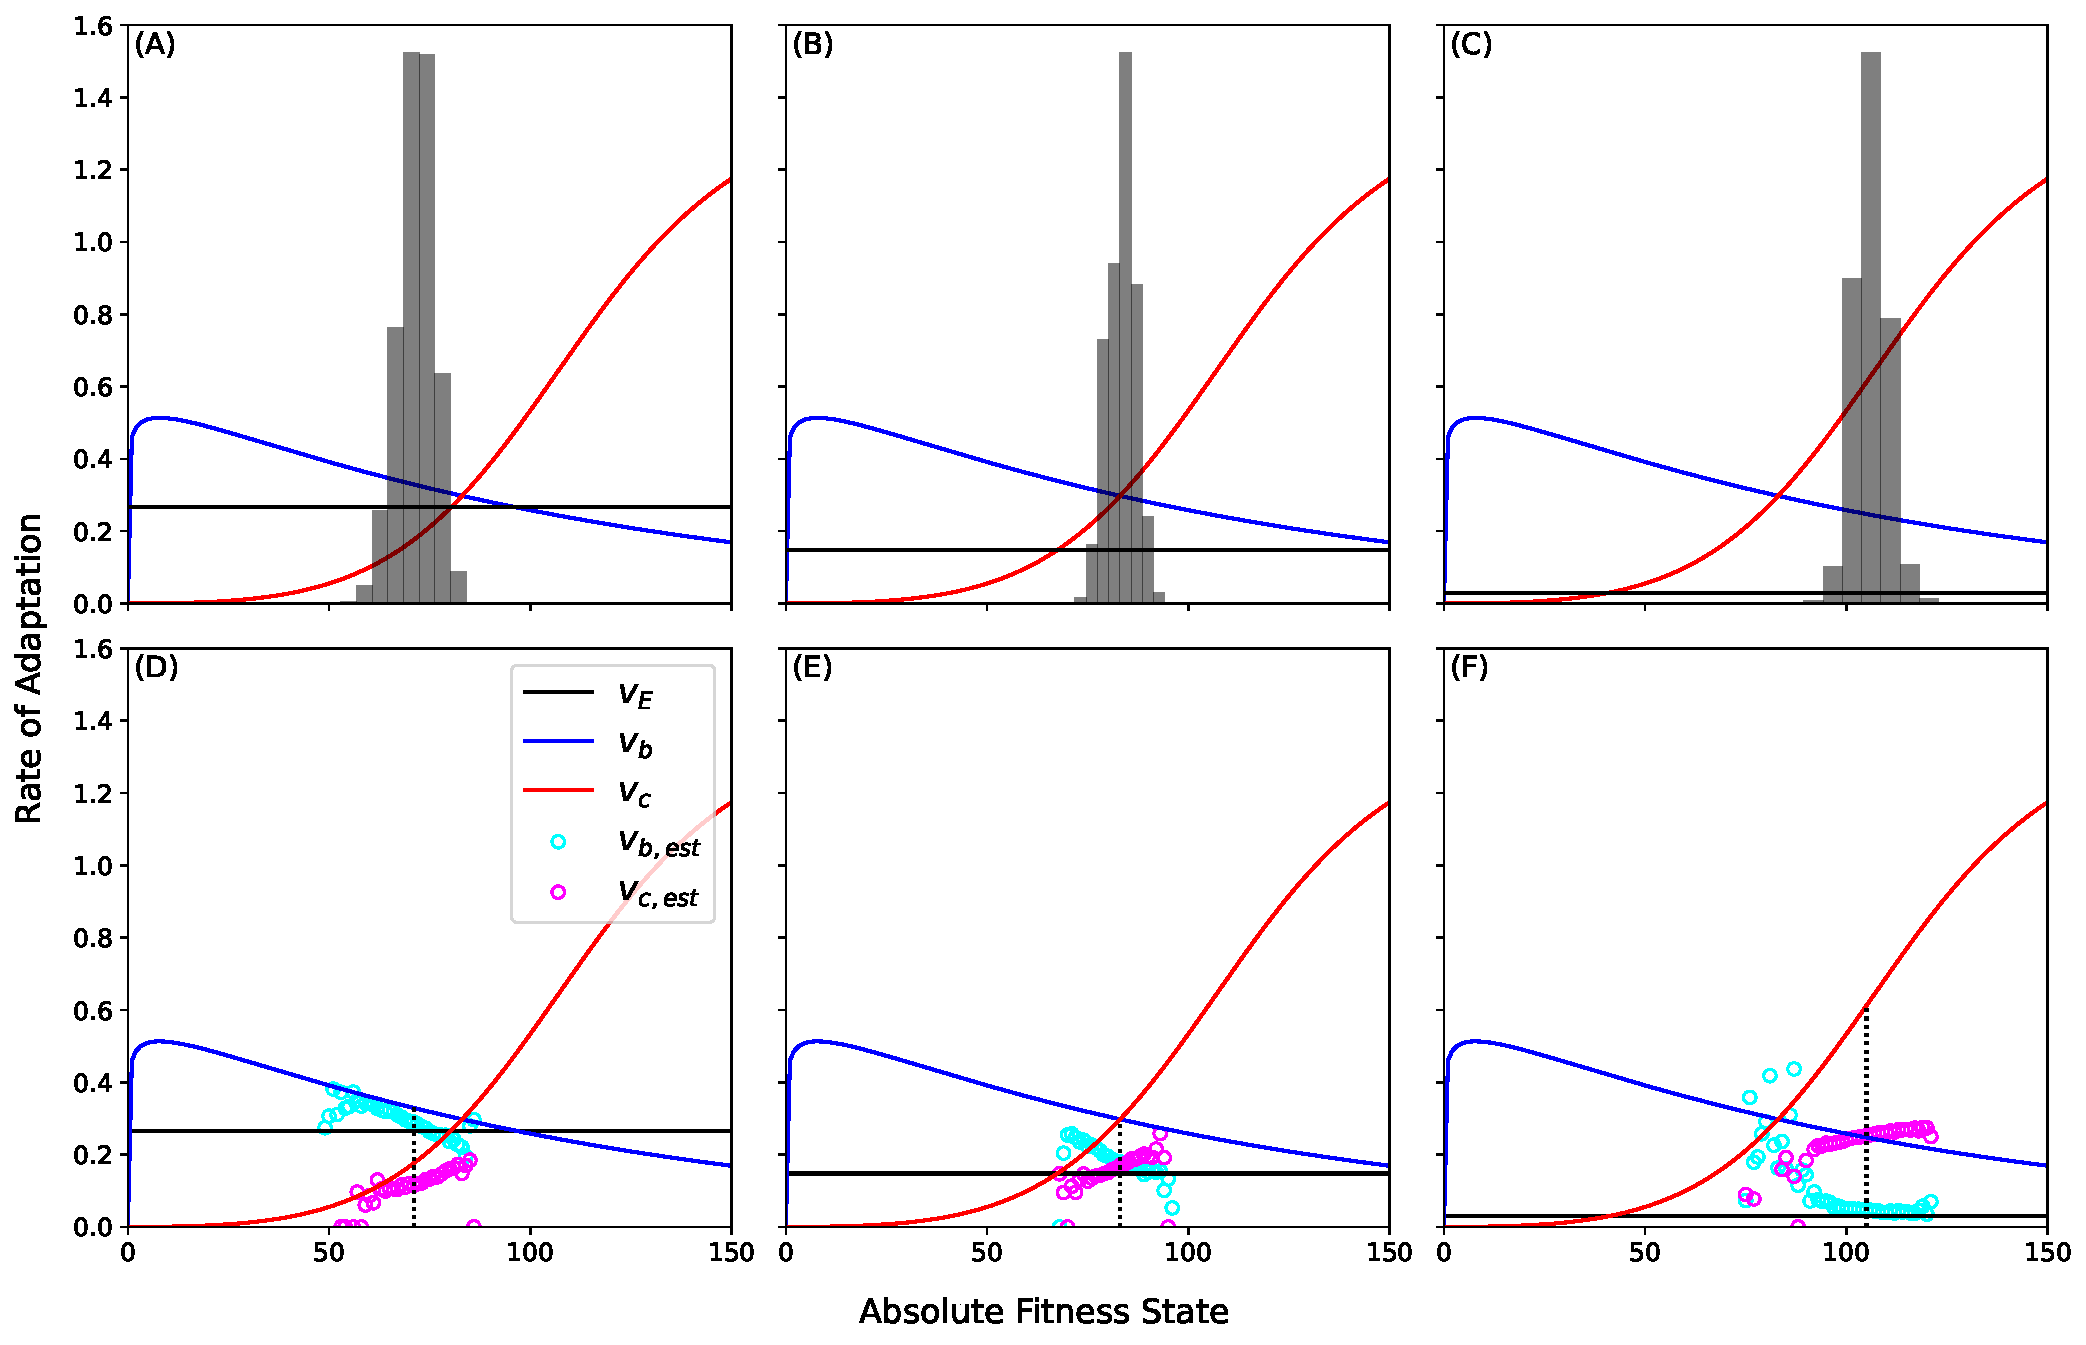
\includegraphics[scale=.60]{Fig/Supplement/fig_bEvo_DRE_traitInterference_mcPlots_pnlC.pdf}
    \caption{Alternate model parameters demonstrate  similar degrees of stalling in the case of  $\rho$ exceeding 1, and weaker diminishing returns epistasis. (A-E) include estimates rates of adaptation, while (F-J) provide histograms showing sojourn times of the population mean fitness state. In all panels, $\rho=1.12$, $T=10^9$, $d=1.2$, $U_b=5\times10^{-6}$, $U_c=5\times10^{-6}$, $s_{b,0}=0.02$, $\alpha=0.995$, and $c_{+}=0.02$.}
    \label{fig:supp:mcSimEst_highRho}
\end{figure}
\vspace*{\fill}\clearpage
\end{landscape}

\newpage
\vspace*{\fill}
\begin{figure}[!h]
    \centering
    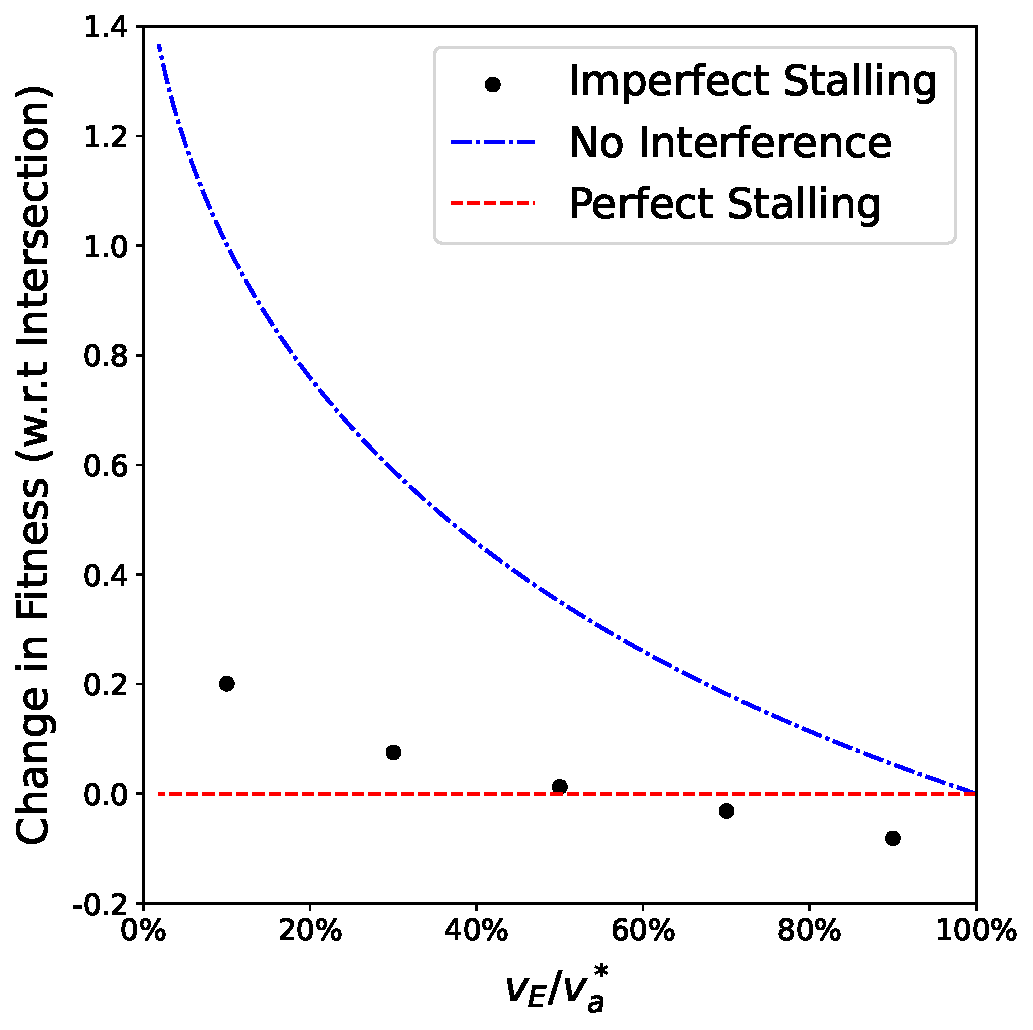
\includegraphics[scale=.62]{Fig/Supplement/fig_bEvo_DRE_traitInterference_fitnessGain_rho1.pdf}
    \caption{The imperfect nature of stalling has a relatively small effect on the sensitivity of population fitness to habitat size $T$.}
\label{fig:supp:mcSimEst_smallRho}
\end{figure}
\vspace*{\fill}\clearpage

\newpage
\begin{landscape}
\vspace*{\fill}
\begin{figure}[!h]
    \centering
    \includegraphics[scale=.62]{Fig/Supplement/fig_bEvo_DRE_traitInterference_increaseT_rho1.pdf}
    \caption{}
\label{fig:supp:mcSimEst_smallRho}
\end{figure}
\vspace*{\fill}\clearpage
\end{landscape}

\end{document}


